%%%%%%%%%%%%%%%%%%%%%%%%%%%%%%%%%%%%%%%%%
% Short Sectioned Assignment
% LaTeX Template
% Version 1.0 (5/5/12)
%
% This template has been downloaded from:
% http://www.LaTeXTemplates.com
%
% Original author:
% Frits Wenneker (http://www.howtotex.com)
%
% License:
% CC BY-NC-SA 3.0 (http://creativecommons.org/licenses/by-nc-sa/3.0/)
%
%%%%%%%%%%%%%%%%%%%%%%%%%%%%%%%%%%%%%%%%%

%----------------------------------------------------------------------------------------
%	PACKAGES AND OTHER DOCUMENT CONFIGURATIONS
%----------------------------------------------------------------------------------------

\documentclass[letterpaper, fontsize=11pt]{scrartcl} % A4 paper and 11pt font size

\usepackage[T1]{fontenc} % Use 8-bit encoding that has 256 glyphs
\usepackage{fourier} % Use the Adobe Utopia font for the document - comment this line to return to the LaTeX default
\usepackage[english]{babel} % English language/hyphenation
\usepackage{amsmath,amsfonts,amsthm} % Math packages

\usepackage{lipsum} % Used for inserting dummy 'Lorem ipsum' text into the template
\usepackage[margin=1in]{geometry} %set margins -TA
\usepackage{sectsty} % Allows customizing section commands
\allsectionsfont{\centering \normalfont\scshape} % Make all sections centered, the default font and small caps
\usepackage{enumitem}
\usepackage{fancyhdr} % Custom headers and footers
\usepackage{graphicx}
\pagestyle{fancyplain} % Makes all pages in the document conform to the custom headers and footers
\fancyhead{} % No page header - if you want one, create it in the same way as the footers below
\fancyfoot[L]{\textit{CME 102 Winter '17-'18}} % Empty left footer
\fancyfoot[C]{} % Empty center footer
\fancyfoot[R]{Tim Anderson} % Page numbering for right footer
\renewcommand{\headrulewidth}{0pt} % Remove header underlines
\renewcommand{\footrulewidth}{0pt} % Remove footer underlines
\setlength{\headheight}{14pt} % Customize the height of the header

\allowdisplaybreaks

\numberwithin{equation}{section} % Number equations within sections (i.e. 1.1, 1.2, 2.1, 2.2 instead of 1, 2, 3, 4)
\numberwithin{figure}{section} % Number figures within sections (i.e. 1.1, 1.2, 2.1, 2.2 instead of 1, 2, 3, 4)
\numberwithin{table}{section} % Number tables within sections (i.e. 1.1, 1.2, 2.1, 2.2 instead of 1, 2, 3, 4)

\setlength\parindent{0pt} % Removes all indentation from paragraphs - comment this line for an assignment with lots of text
\begin{document}

%----------------------------------------------------------------------------------------
%	TITLE SECTION
%----------------------------------------------------------------------------------------

\newcommand{\horrule}[1]{\rule{\linewidth}{#1}} % Create horizontal rule command with 1 argument of height

%----------------------------------------------------------------------------------------
%	PROBLEM 1
%----------------------------------------------------------------------------------------

\section*{Week 9 Section Solutions}
\par If not otherwise specified, solve the following problems. If initial conditions are given, solve for all constants of integration. It is okay to leave answers in implicit form or with unsolved integrals. 
\begin{enumerate}
\item \textbf{Getting to know your Laplace Transform} \newline Remember the mathematical definition of the Laplace transform:
$$ \mathcal{L}\{f(t)\} = F(s) = \int_0^\infty f(t)e^{-st}dt$$
Using this, derive the following properties of the Laplace transform. \textit{Hint:} you will need to use substitution and integration by parts liberally.
\begin{enumerate}

\item \textit{s-Shift} $ \mathcal{L}\{e^{at}f(t)\} = F(s-a)$ \newline
\textbf{Solution:} 
$$\mathcal{L}\{e^{at}f(t)\} = \int_0^\infty e^{at}f(t)e^{-st}dt = \int_0^\infty f(t)e^{-st+at}dt = \int_0^\infty f(t)e^{-t(s-a)}dt$$
$$\text{Substituting $s' = s-a$: } \int_0^\infty f(t)e^{-ts'}dt = F(s') = F(s-a)$$

\item \textit{t-Shift} $ \mathcal{L}\{u(t-a)f(t-a)\} = e^{-as}F(s)$ \newline
\textbf{Solution:}
$$\mathcal{L}\{u(t-a)f(t-a)\} = \int_0^\infty u(t-a)f(t-a)e^{-st}dt = \int_a^\infty f(t-a)e^{-st}dt$$
Substituting $\tau = t-a$ and changing the bounds of integration:
$$\int_0^\infty f(\tau)e^{-s(\tau+a)}dt = \int_0^\infty f(\tau)e^{-s\tau}e^{-as}dt = e^{-as}\int_0^\infty f(\tau)e^{-s\tau}dt = e^{-as}F(s)$$

\item \textit{Derivative identity} For some function $f(t)$, $ \mathcal{L}\{f'(t)\} = sF(s) - f(0)$ \newline
\textbf{Solution:}
$$\mathcal{L}\{f'(t)\} = \int_0^\infty f'(t)e^{-st}dt$$
Remember integration by parts: $\int udv = uv - \int vdu$. Take $u = e^{-st}$ and $v=f(t)$, then:
$$ \int_0^\infty f'(t)e^{-st}dt = f(t)e^{-st}\Big{|}_0^\infty - \int_0^\infty f(t)(-se^{-st})dt$$ 
$$= \lim_{t\to\infty} f(t)e^{-st} - f(0)e^{-s(0)} + s\int_0^\infty f(t)e^{-st}dt = sF(s) - f(0)$$

\end{enumerate}

\item \textbf{Warm-up} Solve the following ODE using a Laplace transform. \newline
$$y'' + 2y' + y = sin(t), \quad y(0) = 0, \quad y'(0) = 0$$
\textbf{Solution:} Take the Laplace transform:
$$s^2Y(s) - sy(0) - y'(0) + 2sY(s) - 2y(0) + Y(s) = \frac{1}{s^2 + 1}$$
$$\text{Applying initial condiitons: } s^2Y(s) + 2sY(s) + Y(s) = \frac{1}{s^2 + 1}$$
$$Y(s)(s^2 + 2s + 1) = Y(s)(s+1)^2 = \frac{1}{s^2 + 1} $$
$$Y(s) = \frac{1}{(s^2 + 1)(s+1)^2} = \frac{-s}{2(s^2 + 1)} + \frac{1}{2(s+1)} + \frac{1}{2(s+1)^2}$$
$$y(t) = \frac{-1}{2}cos(t) + \frac{1}{2}e^{-t}t + \frac{1}{2}e^{-t}$$
Were you not to use a Laplace transform, which methods could you use instead to solve this ODE? Which of these methods (including Laplace transform) do you think is the easiest? \par
\textbf{Solution:} You could also solve this  using \textit{variation of parameters} or \textit{undetermined coefficients}. All of these methods have their upsides and downsides, but Laplace transforms are probably the easiest method for solving a problem of this form. However, it comes down to personal preference.

\item \textbf{Laplace transform with impulse input} Suppose you have a mass-spring system governed by the following equation:
$$y'' + 4y' + 5y = \delta(t-3)$$ where $\delta(t-a)$ is a shifted Dirac delta function. 
\begin{enumerate}
\item Briefly describe intuitively what is going on in this system. \par
\textbf{Solution:} A delta function represents an impulse. A good physical analogue of a delta would be slapping the mass spring system: it is a very brief impact from an outside source. For this system, it could be someone slapping the spring at time $t = 3$. 
\item Solve for $y(t)$ using the initial conditions $y(0) = 0$, $y'(0) = 0$. \newline
\textbf{Solution:} Since we are dealing with a discrete input, the only way to solve this problem is with Laplace transforms.
$$s^2Y(s) - sy(0) - y'(0) + 4sY(s) - 4y(0) + 5Y(s) = e^{-3s}$$
Applying initial conditions:
$$Y(s)(s^2 + 4s + 5) = e^{-3s}$$
$$Y(s) = \frac{e^{-3s}}{s^2 + 4s + 5} = \frac{e^{-3s}}{s^2 + 4s + 4 - 4 + 5} = \frac{e^{-3s}}{(s+2)^2 + 1} = \frac{e^{-3s}}{((s+2)^2 + 1)}$$
$$y(t) = u(t-3)e^{-2(t-3)}sin(t-3)$$
\item Qualitatively, what does this solution look like when plotted? \par
\textbf{Solution:} The system is at rest at $y(t) = 0$ until time $t = 3$ when the system receives the input and begins oscillating as a decaying sinusoid. A plot is shown below:
\begin{center} 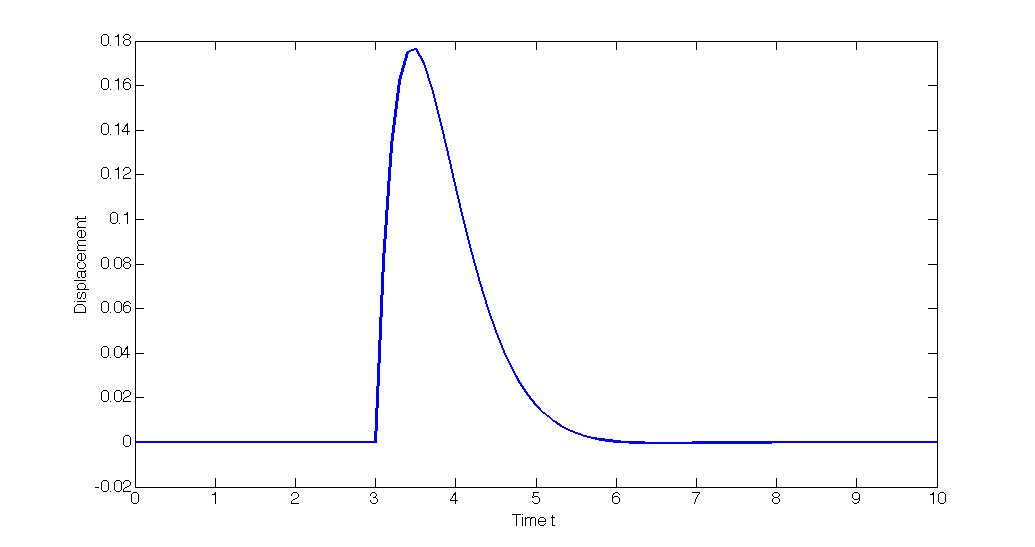
\includegraphics[width = 4.2in]{section9_2.jpg} \end{center}
\end{enumerate}

\item \textbf{Laplace transform with discrete input} 
\par Solve the following ODEs using Laplace transform. Also sketch a graph of the right-hand-side forcing function (i.e. $f(t)$ in each problem). 
\begin{enumerate}
\item 
% Kryszig 6.3 #24 
$$y'' + 3y' + 2y = f(t),\qquad y(0) = y'(0) = 0$$  
where $f(t) = 1$ for $0 < t < 1$ and $f(t) = 0$ for $t > 1$. 
\par \textbf{Solution:}\newline
We first need to re-express the piece-wise function $f(t)$ in terms of Heaviside step functions:

\[ 
f(t) = \begin{cases} 
      1 & 0 < t < 1 \\
      0 & t > 1 
   \end{cases}
   \implies
   f(t) = 1 - u(t-1)
\]
So we can rewrite the ODE as $y'' + 3y' + 2y = 1 - u(t-1)$. Now, we can solve the ODE using a Laplace transform:
\begin{align*}
y'' + 3y' + 2y &= 1 - u(t-1)\\
s^2 Y(s) - sy(0) - y'(0) + 3sY(s) - 3y(0) + 2Y(s) &= \frac{1}{s} - \frac{e^{-s}}{s}\\
s^2 Y(s) - s(0) - (0) + 3sY(s) - 3(0) + 2Y(s) &= \frac{1}{s} - \frac{e^{-s}}{s}\\
s^2 Y(s) + 3sY(s) + 2Y(s) &= \frac{1}{s} - \frac{e^{-s}}{s}\\
Y(s)\left(s^2 + 3s + 2\right) &= \frac{1}{s} - \frac{e^{-s}}{s}\\
Y(s) &= \left(1 - e^{-s}\right) \left( \frac{1}{s(s^2 + 3s + 2)}\right)\\
Y(s) &= \left(1 - e^{-s}\right) \left( \frac{1}{s(s+2)(s+1)}\right)
\end{align*}
Now, we need to do a partial fraction decomposition:
\begin{align*}
Y(s) &= \left(1 - e^{-s}\right) \left( \frac{1}{s(s+2)(s+1)}\right)\\
&= \left(1 - e^{-s}\right) \left(\frac{A}{s} + \frac{B}{s+2} + \frac{C}{s+1}\right)\\
1&= A\left(s^2 + 3s + 2 \right) + B \left(s^2 + s \right) + C \left(s^2 + 2s\right) \\
1&= s^2 ( A + B + C) + s(3A + B + 2C) + 2A \\
\begin{array}{c}
1 = 2A \\
0 = 3A + B + 2C \\
0 = A + B + C
\end{array}
&\implies
\begin{array}{c}
A = \frac{1}{2} \\
B = \frac{1}{2}\\
C = -1
\end{array} \\
Y(s) &= \left(1 - e^{-s}\right) \left(\frac{1}{2s} + \frac{1}{2(s+2)} - \frac{1}{s+1}\right)\\
y(t) &= \frac{1}{2} + \frac{1}{2}e^{-2t} - e^{-t} -u(t-1)\left(\frac{1}{2} + \frac{1}{2}e^{-2(t-1)} - e^{-(t-1)}\right)\\
\end{align*}


% Kryszig 6.3 #25 
\item $$y'' + y = f(t),\qquad y(0) = y'(0) = 0$$  
where $f(t) = t$ for $0 < t < 1$ and $f(t) = 0$ for $t > 1$. 
\par \textbf{Solution:}\newline
Te-express $f(t)$ in terms of Heaviside step functions:

\[ 
f(t) = \begin{cases} 
      t & 0 < t < 1 \\
      0 & t > 1 
   \end{cases}
   \implies
   f(t) = (1 - u(t-1))t
\]

From here we can solve with Laplace transform:

\begin{align*}
y'' + y &= (1-u(t-1))t\\
&= t- u(t-1)(t-1 + 1)\\
&= t- u(t-1)(t-1) -u(t-1)\\
s^2Y(s)  - sy(0) - y'(0) + Y(s) &= \frac{1}{s^2} - \frac{e^{-s}}{s^2} - \frac{e^{-s}}{s}\\
s^2Y(s) + Y(s) &= \frac{1}{s^2} - \frac{e^{-s}}{s^2} - \frac{e^{-s}}{s} \\
Y(s)\left(s^2 + 1 \right) &=  \frac{1}{s^2}\left(1 - e^{-s}\right) - \frac{e^{-s}}{s}  \\
Y(s) &= \left(1 - e^{-s} \right)\frac{1}{s^2(s^2 + 1)} - \frac{e^{-s}}{s(s^2 + 1)}\\
\end{align*}
We must do partial fractions on both of these fractions as follows:
\begin{align*}
\frac{1}{s^2(s^2 + 1)} &= \frac{A}{s} + \frac{B}{s^2} + \frac{Cs + D}{s^2 + 1}\\
1&= A(s^3 + s) + B(s^2+1) + Cs^3 + Ds^2\\
&= s^3(A + C) + s^2(B + D) + As + B\\
\begin{array}{c}
1 = B \\
0 = A \\
0 = B+D\\
0 = A + C
\end{array}
&\implies
\begin{array}{c}
A = 0 \\
B = 1 \\
C = 0 \\ 
D = -1
\end{array} \\
\frac{1}{s^2(s^2 + 1)} &= \frac{1}{s^2} - \frac{1}{s^2 + 1} \quad \blacksquare\\
\frac{1}{s(s^2 + 1)} &= \frac{A}{s} + \frac{Bs + C}{s^2 + 1}\\
1&= A(s^2 + 1) + Bs^2 + Cs\\
&= s^2(A + B) + Cs + A\\
\begin{array}{c}
1 = A \\
0 = C \\
0 =A + B
\end{array}
&\implies
\begin{array}{c}
A = 1 \\
B = -1 \\
C = 0 
\end{array} \\
\frac{1}{s(s^2 + 1)} &= \frac{1}{s} - \frac{s}{s^2 + 1}\quad\blacksquare\\
\end{align*}

Finally, we can use these partial fractions to find our final solution:
\begin{align*}
Y(s) &= \left(1 - e^{-s} \right)\frac{1}{s^2(s^2 + 1)} - \frac{e^{-s}}{s(s^2 + 1)}\\
&= \left(1 - e^{-s} \right)\left(\frac{1}{s^2} - \frac{1}{s^2 + 1} \right) - e^{-s}\left(\frac{1}{s} - \frac{s}{s^2 + 1}\right)\\
&= \left(\frac{1}{s^2} - \frac{1}{s^2 + 1} \right) - e^{-s}\left(\frac{1}{s^2} - \frac{1}{s^2 + 1} + \frac{1}{s} - \frac{s}{s^2 + 1}\right)\\
y(t) &= t - \sin(t) - u(t-1)\left( (t-1) - \sin(t-1) + 1 - \cos(t-1)\right)\\
 &= t - \sin(t) - u(t-1)\left( t - \sin(t-1) - \cos(t-1)\right)\\
 &= (1-u(t-1))t + u(t-1)(\sin(t-1) + \cos(t-1)) - \sin(t) \quad \blacksquare
\end{align*}

\end{enumerate}


\end{enumerate}

%----------------------------------------------------------------------------------------





\end{document}